One of the algorithm in meta reinforcement learning is the meta-gradient reinforcement learning introduced in \cite{meta-gradient} by Google DeepMind. In deep reinforcement learning, the environment model is often unknown to the agent. Therefore, the true value function has to be approximated by a function known as \textit{return} with parameter $\theta$. This return function plays an important role in determining the characteristics of the reinforcement learning algorithm. Usually, the return function is parameterised by a discount factor $\gamma$ and the bootstrapping parameter $\lambda$. In \cite{meta-gradient}, it is defined as shown below:

\begin{math}
	\begin{aligned}
		G_\eta^{(n)}(\tau_t) &= R_{t+1} + \gamma R_{t+2} + \dots + \gamma^{n-1}R_{t+n} + \gamma^n v_\theta(s_{t+n})\\
		G_\eta^{\lambda}(\tau_t) &= (1-\lambda) \sum_{n=1}^\infty \lambda^{n-1} G_\eta^{(n)}
	\end{aligned}
\end{math}

The two parameters are hand-selected and held fixed throughout training. In \cite{meta-gradient}, these parameters are denoted by $\eta = \{\gamma, \lambda\}$ and $\theta$ is updated by the following formula, taking $\eta$ into account:

\[\theta' = \theta + f(\tau, \theta, \eta)\]

where $\tau$ is the sample of experience being considered.

\par
In order to achieve better performance, $\eta$ is also updated in the training process. A meta-objective defined as follows is used to define the rule to update $\eta$:

\[\bar{J}(\tau', \theta', \bar{\eta}) = (g_{\bar{\eta}}(\tau') - v_\theta'(S'))^2\]

where $\tau'$ is the next sample and $\theta'$ is the updated parameter $\theta$.

$\Delta\eta$ is defined below:

\[\Delta \eta = -\beta \frac{\partial \bar{J}(\tau', \theta', \bar{\eta})}{\partial \theta'} \frac{\partial f(\tau, \theta, \eta)}{d\eta}\]

where $\beta$ is the learning rate for updating $\eta$.

\par
The validation of meta-gradient algorithm is executed on Arcade Learning Environment with an agent built with the IMPALA framework. The agents are evaluated on 57 different Atari games. The result is shown below:
\begin{figure}[H]
	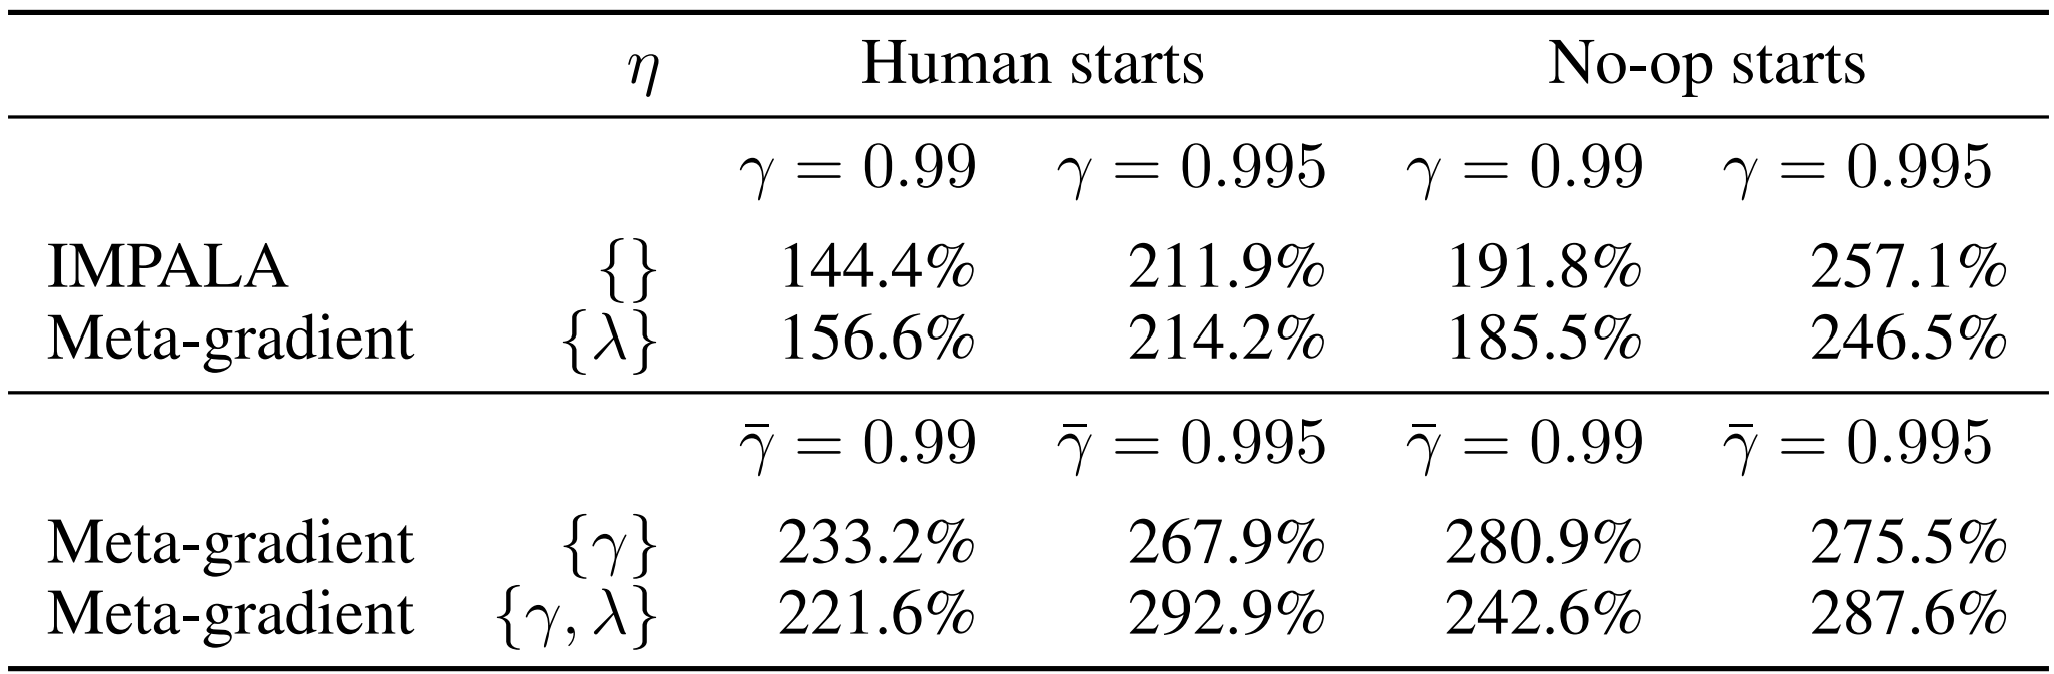
\includegraphics[scale=0.3]{meta-gradient-result.png}
	\centering
	\caption{Experiment result of meta-gradient algorithm. "Human starts" means episodes are initialized to a state that is randomly sampled from human play, while "No-op starts" means each episode is initialized with a random sequence of no-op actions.}
	\label{meta-gradient-result}
\end{figure}
% 
% 
% 